%  ALU.tex
%  Document created by seblovett on seblovett-Ubuntu
%  Date created: Tue 01 Apr 2014 20:10:56 BST
%  <+Last Edited: Fri 04 Apr 2014 15:27:38 BST by hl13g10 on octopus +>


\section{ALU}

\subsection{Design}
The arithmetic logic unit (ALU) is a key part of a processor. 
It is a combinational block, responsible for the arithmetic and logic operations on the data.
The ALU in this processor has three operations on two operands.
No flags, such as carry or zero, are implemented either as no conditional branches are needed.

The ALU supports the operations in table \ref{tab:aluops}.
The operation encodings are discussed in section \ref{sect:controller}.
Due to the use of fixed point notation, the integer result of the multiplication is located at bits [14:7] of the 16 bit result.
To correctly synthesise combinational logic, all inputs must have a defined output.
The ALU was smallest in size when the A function was repeated in the redundant state.

\begin{table}
\caption{ALU Operations supported}
\label{tab:aluops}
\begin{tabular}{|c|c|c|} \hline
Operation & Explanation & Encoding (binary)\\  \hline
A & Result = Operand1 & 00, 10 \\
Add & Result = Operand1 + Operand2 & 01 \\
Multiply & Result = (Operand1 $\times$ Operand2)[14:7] & 11 \\ \hline
\end{tabular}
\end{table}


The Cyclone IV FPGA has a number of embedded multipliers. 
One of these is utilised within the ALU to conduct signed multiplication. 
This is done by defining the inputs as signed, and using a combinational assign statement.
The Quartus tool then recognises this and synthesises the design using the embedded multipliers.
%The multiplier cell also includes 3 registers which are not utilised in this design.


%\todo[inline]{Operations implemented}
%\todo[inline]{Embedded multiplier(s)}
%\todo[inline]{Explain Test bench}

\subsection{Testbench}

The testbench tests each operation with ten different values of the operands. 
An assertion then checks each result is as expected. 
An error count is kept and the simulation is successful if this is zero at the end of the simulation.
Figure \ref{fig:alusim} shows the waveform for the simulation. 
It can be seen that all three operations are tested and the error count is zero at the end. 
The fourth, undefined operation is not tested as the result does not matter. 

\begin{figure}
\includegraphics[height=\textheight]{Figures/alusim.eps}
\caption{Simulation waveform for the ALU testbench}
\label{fig:alusim}
\end{figure}

%\todo[inline]{Simulation results}
%\todo[inline]{Synthesis}
\subsection{Synthesis}

Synthesis of the ALU largely consists of multiplexors. 
As three operations are implemented, this requires 8 3:1 multiplexors. 
There is also an adder and a multiplier. 
The multiplier implemented utilised the embedded multipliers available on the device.

\begin{figure}
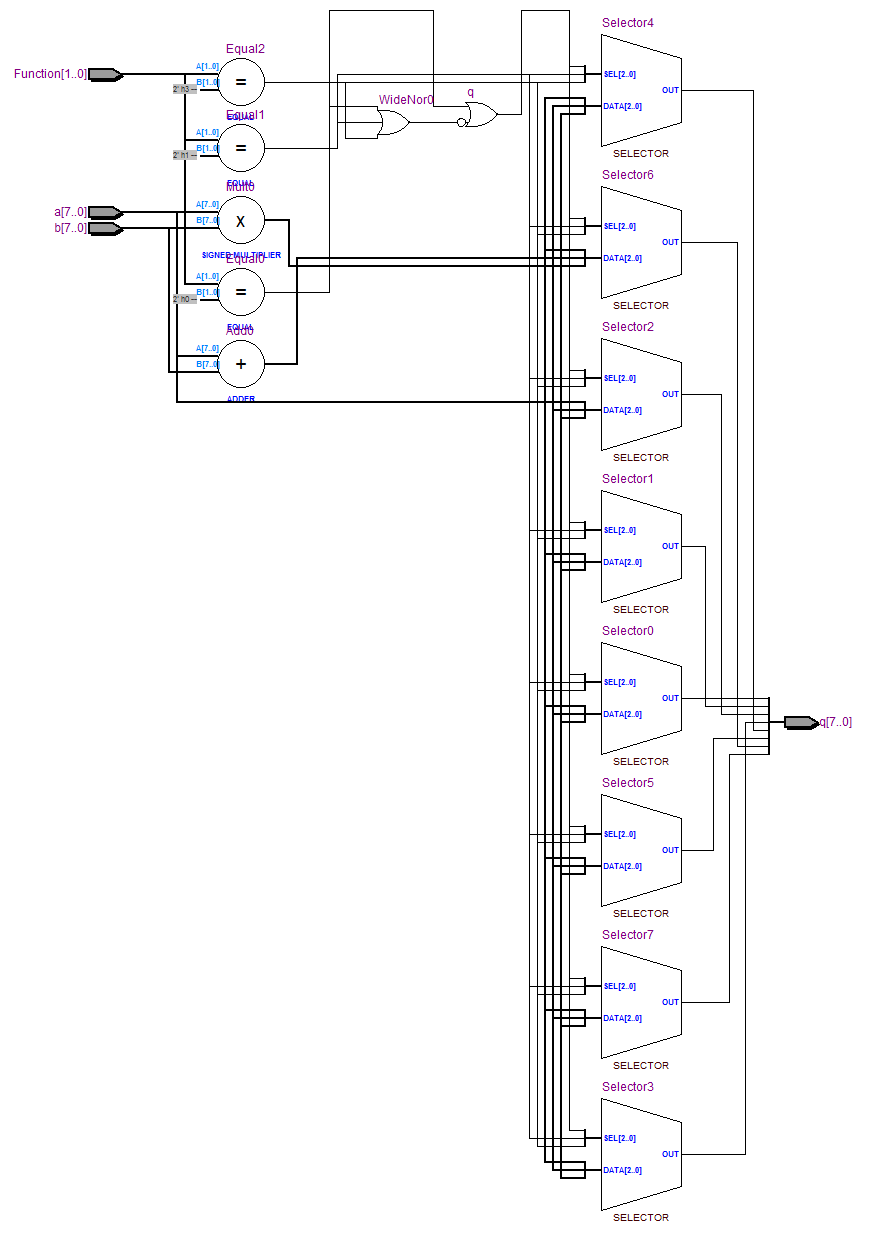
\includegraphics[height=\textheight]{Figures/alusynth.png}
\caption{Synthesis of the Arithmetic Logic Unit}
\label{fig:alusynth}
\end{figure}
